\chapter{Evaluation of \glsentrytext{bosss} for Viscid Flows}
\label{viscousCylinder}
In this chapter we aim at validating \gls{bosss} for viscid flows with \gls{ibm}s. In order to have a good comparable result, we will once again regard the flow around a cylinder as in chapter \cref{eulerVerification}. 
The viscous flow around a cylinder has been approached by many papers both experimentally and numerically, e.g. \cite{williamson1996vortex}, \cite{FLM:14223}, \cite{canutoTaira}, though very few numerical approaches use a \gls{rkdg} method combined with immersed boundaries. In order to verify the \gls{bosss} code with immersed boundaries not only for the Euler equations as we did in chapter \cref{eulerVerification} but also for the viscous case we will now consider different Reynolds numbers for the steady and unsteady flow and compare our results to those of other studies.

\section{Theory}
	The flow around a viscous cylinder can be divided into different sections depending on the Reynolds number as shown in \cref{fig:overview}. The first section applies for Reynolds numbers $0 < \text{Re} < 40-50$ characterised by a laminar steady flow. In that regime a recirculation region with two symmetric vortices with opposite directions is comprised by the wake. The flow can be described using the wake separation length $W^*$.\\\\
	\begin{figure}[htp]
		\centering
		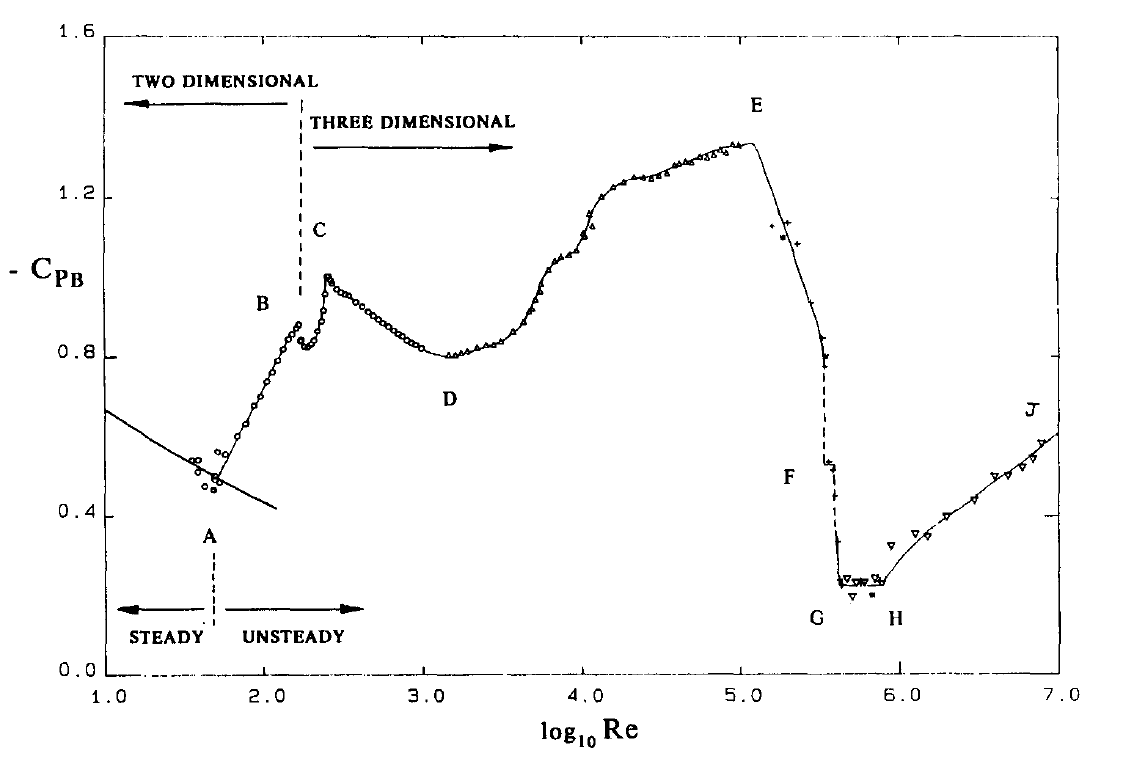
\includegraphics[height=8cm]{overviewCylinderReynolds_Williamson.PNG}
		\caption{Overview of Base Suction Coefficients over Reynolds Number \cite{williamson1996vortex}}
		\label{fig:overview}
	\end{figure} 
	The second section contains all other Reynolds number $\text{Re}> 40-50$ and thus describes the unsteady flow. It can be subdivided in several subsections \cite{williamson1996vortex}:
	\begin{description}
		\item[$40-50 < \text{Re} < 190$] laminar vortex shedding,
		\item[$190 < \text{Re} < 260$] \gls{3d} wake-transition regime,
		\item[$260 < \text{Re} < 1000$] increasing disorder in the fine-scale three dimensionalities,
		\item[$1000 < \text{Re} < 200000$] shear layer transition regime,
		\item[$200000 < \text{Re}$] critical transition, supercritical regime and post-critical regime.
	\end{description}
	
	As we will only discuss Reynolds numbers up to $\text{Re} = 200$ the important phases for us are the laminar steady regime and the laminar vortex shedding. At around $\text{Re} = 190$ the three dimensionality of the system has an incrementing influence on the flow; for we only analyse the 2-D model of the experiment we stop at $\text{Re} = 200$ expecting slight deflection in our results.
	
	\subsection{The Laminar Steady Regime}
	
	At Reynolds numbers below 50 the flow forms a steady recirculation region, characterised by the wake separation length  $W^*$. It is built by two symmetrically placed vortices on each side of the wake as can be seen in \cref{fig:steady}. It has been shown experimentally as well as numerically, that the wake separation length increases with increasing Reynolds number. 
		\begin{figure}[htp]
			\centering
			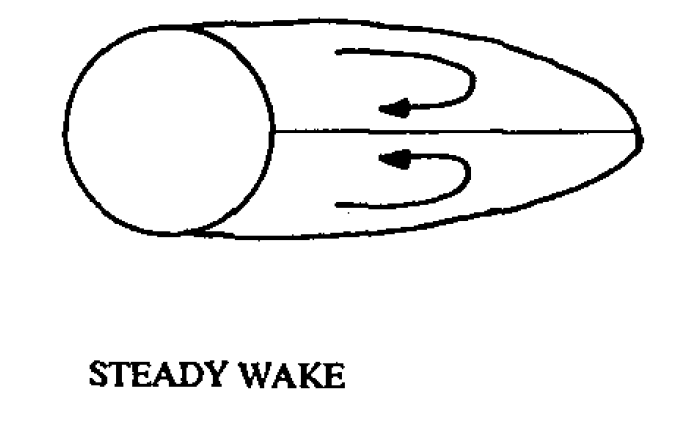
\includegraphics[height=4cm]{steadyFlow_Williamson.PNG}
			\caption{Recirculation Region \cite{williamson1996vortex}}
			\label{fig:steady}
		\end{figure}
	\subsection{Laminar Vortex Shedding}
	For Reynolds numbers of between 50 and 200 the recirculation region develops instabilities leading to the development of turbulence in the wake. This results into fully periodic vortex shedding, known as the Kármán vortex street, as can be seen in \cref{fig:unsteady}. With increasing Reynolds number the amplitudes of drag and lift coefficients increases while the Strouhal number and frequency, respectively, decreases.
	
		\begin{figure}[htp]
			\centering
			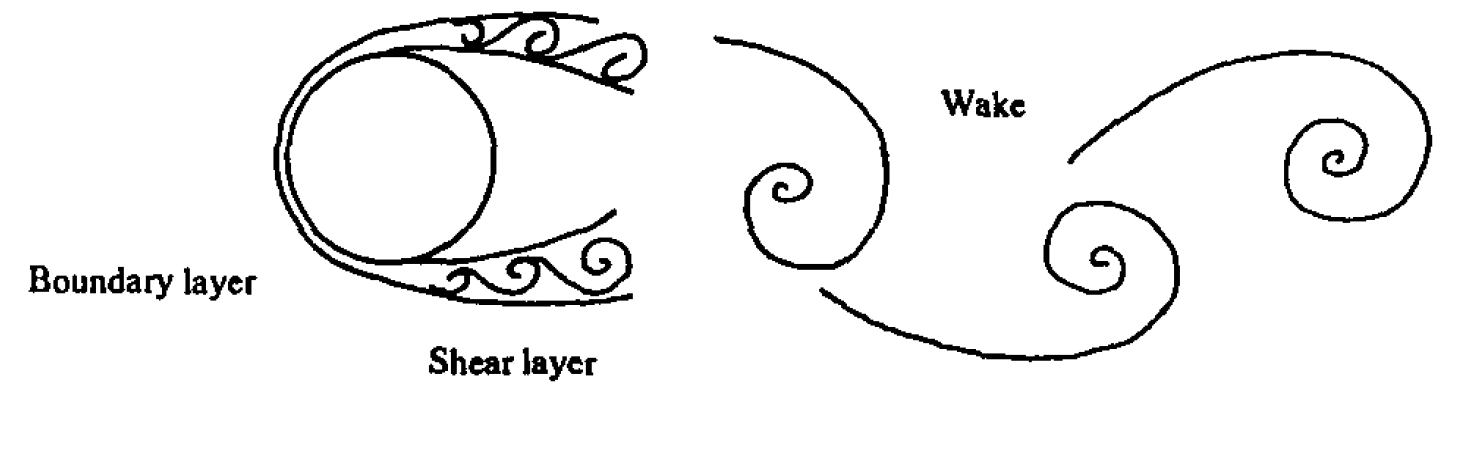
\includegraphics[height=4cm]{unsteady_Williamson.PNG}
			\caption{Kármán Vortex Street \cite{williamson1996vortex}}
			\label{fig:unsteady}
		\end{figure}
		
\section{Simulations}
	In this section we will compare the lift and drag coefficients $C_L$ and $C_D$ at different Reynolds numbers and mesh sizes at a constant agglomeration threshold of $0.3$, different polynomial degrees of 1, 2 and 3 and meshes of $40 \times 40$, $80 \times 80$ and $160 \times 160$ cells. These mesh sizes were developed from 32, 64 and 128 cells per direction but overlaying them with a mesh with one eighth of those in order to better approach the boundary layer of the cylinder. The meshes can be found in the appendix. \\\indent
	The different simulation properties will be abbreviated as DG $+$ \textit{polynomial degree} $+$ CpD $+$ \textit{number of cells per direction}, e.g. DG2CpD80 for a simulation with polynomial degree 2 and $80 \times 80$ cells.\\
	 The drag and lift coefficients are defined as
	\begin{align}
		C_D = \dfrac{d}{q_\infty L_\infty} \\
		C_L = \dfrac{l}{q_\infty L_\infty}
	\end{align}
	with the dynamic pressure $q_\infty = \dfrac{1}{2} \rho_\infty V_\infty^2$. For we set $L_\infty = \rho_\infty = V_\infty = 1$ in our boundary and initial conditions, we can assume
	\begin{align}
		C_D = 2 \cdot d \\
		C_L = 2 \cdot l,
	\end{align}
	with the drag and lift forces $d$ and $l$ provided from the calculation. \\\\
	During the simulations we now compute the complete domain with $-40 \leq x \leq 40$, $-40 \leq y \leq 40$ and the cylinder radius $r = 1$ as we expect asymmetrical oscillations of the flow with higher Reynolds numbers.
	We will use a rectilinear mesh that is finer near the cylinder, an isothermal wall boundary condition at the cylinder wall and supersonic inlet boundary conditions for the domain borders that shall prevent the reflection of the initial wave.  \\\\
%	For the calculation with DG3CpD40 no results could be found. The case produces a ill conditioned matrix that is not positive definite; thus the Cholesky factorisation fails. We can therefore conclude that it is unsafe to use \gls{bosss} with high order on very coarse meshes. These results match those that we found in \ref{eulerVerification} where we got irregular values for DG3CpD32 during the robustness study.
	
	\subsection{Steady State Simulations ($\text{Re} < 40-50$)}
	For the steady state simulations we can use the wake separation length $W^*$ as an additional variable to compare to other simulations.
			\begin{figure}[htp]
				\centering
				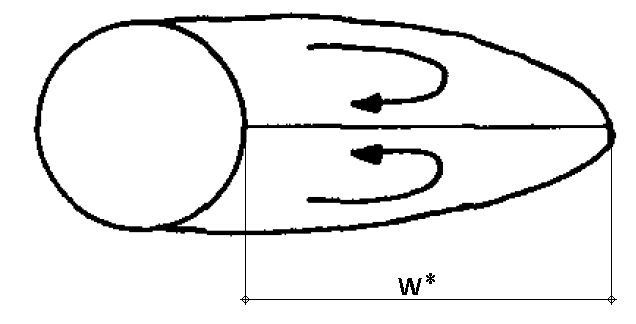
\includegraphics[height=4cm]{steadyFlow_modifiedWilliamson.PNG}
				\caption{Wake separation length, from \cite{williamson1996vortex} modified }
				\label{fig:wakeSeparation}
			\end{figure} 
	It can be found from examining the x-velocity $U$ at $y=0$; the x-position where $U$ changes its sign should be the end position of the wake.
%	\subsubsection{Simulation at Reynolds Number 10}
%
%	\begin{figure}[htp]	
%		\centering
%		\begin{tikzpicture}
%		\begin{semilogxaxis}[xlabel ={Cells per Direction}, ylabel ={$C_D$},  grid =major, legend entries ={$P=1$}, unbounded coords=jump, legend style = {cells = {anchor=east}, legend pos=outer north east,}, scaled x ticks = false, scaled y ticks = false, xmin = 32, xmax = 128, ymax = 2.7]
%		\addplot table[ x = meshSize, y =C_D] {data/re10.dat};
%		\addlegendentry{$P=1$}
%		\addplot[mark=none, red] coordinates {(32, 2.5) (128, 2.5)};
%		\addlegendentry{Constant Value}
%		\end{semilogxaxis}	
%		\end{tikzpicture}
%		\label{shivfjfterror}	
%		\caption{Convergence Plot}
%	\end{figure}
%	
%	\begin{figure}[htp]	
%		\centering
%		\begin{tikzpicture}
%		\begin{semilogxaxis}[xlabel ={Cells per Direction}, ylabel ={$C_L$},  grid =major, legend entries ={$P=1$}, unbounded coords=jump, legend style = {cells = {anchor=east}, legend pos=outer north east,}, scaled x ticks = false, scaled y ticks = false, xmin = 32, xmax = 128]
%		\addplot table[ x = meshSize, y =C_L] {data/re10.dat};
%		\addlegendentry{$P=1$}
%		\addplot[mark=none, red] coordinates {(32, 0) (128, 0)};
%		\addlegendentry{Constant Value}
%		\end{semilogxaxis}	
%		\end{tikzpicture}
%		\label{shivfjftqerror}	
%		\caption{Convergence Plot}
%	\end{figure}
%
%	\begin{table}[htp]
%		\centering
%		\begin{tabular}{|c||c|c|c|c}
%			\cline{1-4}
%			\rule{0pt}{2,3ex}\multirow{2}{*}{}   & \multicolumn{3}{c|}{mesh size} &  \\ \cline{2-4}
%			\rule{0pt}{2,3ex}& $32 \times 32$       & $64 \times 64$       & $128 \times 128$      &  \\ \cline{1-4}
%			\rule{0pt}{2,3ex}$W^*$ 				 & a        & b        & c        &  \\ \cline{1-4}
%			\rule{0pt}{2,3ex}$C_D$                & $2.2763840026747$        & $2.3205402064175$        & $2.41364044322$        &  \\ \cline{1-4}
%			\rule{0pt}{2,3ex}$C_L$                & $-0.00055059425842785$        & $-0.0014617338683891$        & $0.00004720682$        &  \\ \cline{1-4}
%		\end{tabular}
%		\caption{Wake separation length and coefficients of drag and lift for $\text{Re}=10$}
%		\label{tab:re10}
%	\end{table}
	
	\subsubsection{Simulation at Reynolds Number 20}
	We will now simulate the flow at $\text{Re}=20$ and compare our results to several experimental and numerical results as shown in \cref{tab:table20}. The results are divided into three categories: experimental, numerical incompressible and numerical compressible in order to coincide with the arrangement given by \cite{ayers}.

\begin{table}[htp]
	\centering
	\begin{tabular}{|c|l|c|c|c|}
		\hline
		\rule{0pt}{2,3ex}$\text{Re}=20$                              & Source                             & 2D/3D & $W^*$ & $C_D$ \\ \hline
		\rule{0pt}{2,3ex}\multirow{3}{*}{Numerical - Incompressible} & Dennis et al {[}1970{]}            & 2D    & 0.94     & 2.05     \\ \cline{2-5} 
		\rule{0pt}{2,3ex}& Forberg {[}1980{]}                 & 2D    & 0.91     & 2.00     \\ \cline{2-5} 
		\rule{0pt}{2,3ex}& Linnick et al. {[}2005{]}          & 2D    & 0.93     & 2.06     \\ \hline
		\rule{0pt}{2,3ex}\multirow{2}{*}{Experimental}               & Coutanceau et al. {[}1978{]}       & -     & 0.93    & -     \\ \cline{2-5} 
		\rule{0pt}{2,3ex}& Tritton {[}1959{]}                 & -     & -     & 2.09     \\ \hline
		\rule{0pt}{2,3ex}\multirow{3}{*}{Numerical - Compressible}     & Brehm et al. {[}2015{]} (Ma = 0.1) & 3D    & 0.96     & 2.02     \\ \cline{2-5} 
		\rule{0pt}{2,3ex}& Ayers {[}2015{]}                   & 2D    & 0.975     & 2.06     \\ \cline{2-5} 
		\rule{0pt}{2,3ex}& \textbf{Present Results:}                   & 2D    & d     & 4     \\ \hline
	\end{tabular}	
	\caption{Comparison of Results for $W^*$ and $C_D$, taken from \cite{ayers}, modified}
	\label{tab:table20} 
\end{table}


\begin{table}[htp]
	\centering
	\def\arraystretch{1.5}
	\begin{minipage}[b]{0.3\textwidth}	
			\begin{tabular}{|c|c|c|c|c|}
				\hline
				\multicolumn{2}{|c|}{\multirow{2}{*}{$C_D$}} & \multicolumn{3}{c|}{CpD} \\ \cline{3-5} 
				\multicolumn{2}{|c|}{}                       & 40     & 80    & 160    \\ \hline
				\multirow{3}{*}{DG}            & 1           &        &       &        \\ \cline{2-5} 
				& 2           &        &       &        \\ \cline{2-5} 
				& 3           &        &       &        \\ \hline
			\end{tabular}
			\caption[$C_D$ Values for each simulation]{$C_D$ Values for each simulation \newline}	
			\label{C_D20}
	\end{minipage}
	\centering
	\quad
	\begin{minipage}[b]{0.3\textwidth}	
		\begin{tabular}{|c|c|c|c|c|}
			\hline
			\multicolumn{2}{|c|}{\multirow{2}{*}{$W^*$}} & \multicolumn{3}{c|}{CpD} \\ \cline{3-5} 
			\multicolumn{2}{|c|}{}                       & 40     & 80    & 160    \\ \hline
			\multirow{3}{*}{DG}            & 1           &        &       &        \\ \cline{2-5} 
			& 2           &        &       &        \\ \cline{2-5} 
			& 3           &        &       &        \\ \hline
		\end{tabular}
		\caption{Wake Separation Lengths for each simulation}	
		\label{W20}
	\end{minipage}
\end{table}

	\begin{figure}[htp]	
		\centering
		\begin{tikzpicture}
		\begin{semilogxaxis}[xlabel ={Cells per Direction}, ylabel ={$C_D$},  grid =major, legend entries ={$P=1$}, unbounded coords=jump, legend style = {cells = {anchor=east}, legend pos=outer north east,}, scaled x ticks = false, scaled y ticks = false, xmin = 32, xmax = 128, ymax = 2.0]
		\addplot table[ x = meshSize, y =C_D] {data/re20.dat};
		\addlegendentry{$P=1$}
		\addplot[mark=none, red] coordinates {(32, 1.6) (128, 1.6)};
		\addlegendentry{Constant Value}
		\end{semilogxaxis}	
		\end{tikzpicture}
		\caption{Graphical presentation of \cref{C_D20} for Re=20}
		\label{shivfjftersaror}	
	\end{figure}
	

	\subsubsection{Simulation at Reynolds Number 40}
\begin{table}[htp]
	\centering
	\begin{tabular}{|c|l|c|c|c|}
		\hline
		\rule{0pt}{2,3ex}$\text{Re}=40$                              & Source                             & 2D/3D & $W^*$ & $C_D$ \\ \hline
		\rule{0pt}{2,3ex}\multirow{3}{*}{Numerical - Incompressible} & Dennis et al {[}1970{]}            & 2D    & 2.35     & 1.52     \\ \cline{2-5} 
		\rule{0pt}{2,3ex}& Forberg {[}1980{]}                 & 2D    & 2.24     & 1.50    \\ \cline{2-5} 
		\rule{0pt}{2,3ex}& Linnick et al. {[}2005{]}          & 2D    & 2.28     & 1.54     \\ \hline
		\rule{0pt}{2,3ex}\multirow{2}{*}{Experimental}               & Coutanceau et al. {[}1978{]}       & -     & 2.13    & -     \\ \cline{2-5} 
		\rule{0pt}{2,3ex}& Tritton {[}1959{]}                 & -     & -     & 1.59     \\ \hline
		\rule{0pt}{2,3ex}\multirow{3}{*}{Numerical - Compressible}     & Brehm et al. {[}2015{]} (Ma = 0.1) & 3D    & 2.26     & 1.51     \\ \cline{2-5} 
		\rule{0pt}{2,3ex}& Ayers {[}2015{]}                   & 2D    & 2.250     & 1.605     \\ \cline{2-5} 
		\rule{0pt}{2,3ex}& \textbf{Present Results:}                   & 2D    & d     & 4     \\ \hline
	\end{tabular}	
	\caption{Comparison of Results for $W^*$ and $C_D$, taken from \cite{ayers}, modified}
	\label{table40}
\end{table}

	\subsection{Unsteady Simulations ($\text{Re}> 40-50$)}
	In order to compare the unsteady simulations we need the Strouhal number
	\begin{align}
		\text{St} = \dfrac{f  L_\infty}{V_\infty}.
	\end{align}
	As our initial and boundary conditions give $V_\infty = L_\infty = 1$, we can calculate $\text{St} = f$ with $f$ found from examining the oscillation of $C_L$ over time. For developing vortex shedding, the flow needs small perturbations that destabilize the flow towards a symmetry breaking state \cite{FLM:14223}. In reality those are given by the structure of the cylinder, the influence of the walls or the not completely straight inflow; in our simulations they come from small truncation errors and the computer's round-off errors. 
	In order to accelerate the process until the wake begins to oscillate one could also start the flow with a vortex that induces a high perturbation much earlier. For it did not take long until the wake began to oscillate it was not needed in our simulations.
	\subsubsection{Simulation at Reynolds Number 100}
\begin{table}[htp]
	\centering
	\begin{tabular}{|c|p{4cm}|c|c|c|c|}
		\hline
		\rule{0pt}{2,3ex}$\text{Re}=100$                              & Source                             & 2D/3D & $St$ & $C_D$ & $C_L$\\ \hline
		\rule{0pt}{2,3ex}\multirow{7}{*}{Numerical - Incompressible} & Gresho et al. {[}1984{]}            & 2D    & 0.18     & 1.76 & -   \\ \cline{2-6} 
		\rule{0pt}{2,3ex}& Linnick et al. {[}2005{]} \newline ($\lambda = 0.056$)                 & 2D    & 0.169     & 1.38 \plusminus 0.010  &  \plusminus  0.337 \\ \cline{2-6} 
		\rule{0pt}{2,3ex}& Linnick et al. {[}2005{]} \newline ($\lambda = 0.023$)                  & 2D    & 0.169     & 1.34 \plusminus 0.009  &  \plusminus 0.333 \\ \cline{2-6} 
		\rule{0pt}{2,3ex}& Persillon et al. {[}1998{]}                 & 2D    & 0.165     & 1.253  & -  \\ \cline{2-6} 
		\rule{0pt}{2,3ex}& Saiki et al. {[}1996{]}                 & 2D    & 0.171     & 1.26  &  - \\ \cline{2-6} 
		\rule{0pt}{2,3ex}& Persillon et al. {[}1998{]}                 & 3D    & 0.164     & 1.240  & -  \\ \cline{2-6} 
		\rule{0pt}{2,3ex}& Liu et al. {[}1998{]}          & 3D    & 0.165     & 1.35 \plusminus 0.012  & \plusminus 0.339  \\ \hline
		\rule{0pt}{2,3ex}\multirow{2}{*}{Experimental}               & Berger et al. {[}1972{]}       & -     & 0.16-0.17    & -    & -\\ \cline{2-6} 
		\rule{0pt}{2,3ex}& Clift et al. {[}1978{]}                 & -    & -     & 1.24  &  - \\ \cline{2-6} 
		\rule{0pt}{2,3ex}& Williamson {[}1996{]}                 & -     & 0.164    & -   & - \\ \hline
		\rule{0pt}{2,3ex}\multirow{3}{*}{Numerical - Compressible}     & Brehm et al. {[}2015{]} \newline (Ma = 0.1) & 3D    & 0.165     & 1.32 \plusminus 0.01    & \plusminus 0.32 \\ \cline{2-6} 
		\rule{0pt}{2,3ex}& Ayers {[}2015{]}                   & 2D    & 0.167     & 1.371 \plusminus 0.011   & \plusminus 0.333 \\ \cline{2-6} 
		\rule{0pt}{2,3ex}& \textbf{Present Results:}                   & 2D    & d     & 4  &   \\ \hline
	\end{tabular}	
	\caption{Comparison of Results for $St$, $C_D$ and $C_L$, taken from \cite{ayers}, modified}
	\label{table100}
\end{table}
%			\begin{table}[htp]
%				\centering
%				\begin{tabular}{|c||c|c|c|c}
%					\cline{1-4}
%					\rule{0pt}{2,3ex}\multirow{2}{*}{}   & \multicolumn{3}{c|}{mesh size} &  \\ \cline{2-4}
%					\rule{0pt}{2,3ex}& $32 \times 32$       & $64 \times 64$       & $128 \times 128$      &  \\ \cline{1-4}
%					\rule{0pt}{2,3ex}$St$ 				 & a        & b        & c        &  \\ \cline{1-4}
%					\rule{0pt}{2,3ex}$C_D$                & d        & e        & f        &  \\ \cline{1-4}
%					\rule{0pt}{2,3ex}$C_L$                & g        & h        & i        &  \\ \cline{1-4}
%				\end{tabular}
%				\caption{Strouhal number and coefficients of drag and lift for $\text{Re}=100$}
%				\label{tab:re100}
%			\end{table}

	
		\begin{figure}[htp]	
			\centering
			\begin{tikzpicture}
				\begin{axis}[xlabel ={Time}, ylabel ={$C_L$}]%, grid =major, legend entries ={$P=1$}, unbounded coords=jump, legend style = {cells = {anchor=east}, legend pos=outer north east,}, scaled x ticks = false, xmin = 0, xmax = 120]
				\addplot table[ x = time, y = l, mark=none] {data/ms64dg1re100.dat};
				\end{axis}	
			\end{tikzpicture}
			\caption{Lift coefficient over time for Re = 100}
			\label{osci100}	
		\end{figure}
%		\begin{figure}[htp]	
%			\centering
%			\begin{tikzpicture}
%			\begin{axis}[xlabel ={Time}, ylabel ={$C_L$}, grid =major, legend entries ={$P=1$}, unbounded coords=jump, legend style = {cells = {anchor=east}, legend pos=outer north east,}, scaled x ticks = false]
%			\addplot table[ x = time, y = l, mark = none] {data/re100dg1ms128.dat};
%			\end{axis}	
%			\end{tikzpicture}
%			\caption{Convergence Plot}
%			\label{shijfterror}	
%		\end{figure}
%		\begin{figure}[htp]	
%			\centering
%			\begin{tikzpicture}
%			\begin{axis}[xlabel ={Time}, ylabel ={$C_L$},  grid =major, legend entries ={$P=1$}, unbounded coords=jump, legend style = {cells = {anchor=east}, legend pos=outer north east,}, scaled x ticks = false, scaled y ticks = false, xmin = 300, xmax = 350]
%			\addplot table[ x =time, y =l, mark=none] {data/re100dg1ms128.dat};
%			\end{axis}	
%			\end{tikzpicture}
%			\caption{Convergence Plot}
%			\label{shijfterror}	
%		\end{figure}
	\subsubsection{Simulation at Reynolds Number 200}
\begin{table}[htp]
	\centering
	\begin{tabular}{|c|l|c|c|c|c|}
		\hline
		\rule{0pt}{2,3ex}$\text{Re}=100$                              & Source                             & 2D/3D & $St$ & $C_D$ & $C_L$\\ \hline
		\rule{0pt}{2,3ex}\multirow{3}{*}{Numerical - Incompressible} & Dennis et al {[}1970{]}            & 2D    & 0.94     & 2.05 &    \\ \cline{2-6} 
		\rule{0pt}{2,3ex}& Forberg {[}1980{]}                 & 2D    & 0.91     & 2.00  &   \\ \cline{2-6} 
		\rule{0pt}{2,3ex}& Linnick et al. {[}2005{]}          & 2D    & 0.93     & 2.06  &   \\ \hline
		\rule{0pt}{2,3ex}\multirow{2}{*}{Experimental}               & Coutanceau et al. {[}1978{]}       & -     & 0.93    & -    & \\ \cline{2-6} 
		\rule{0pt}{2,3ex}& Tritton {[}1959{]}                 & -     & -     & 2.09   &  \\ \hline
		\rule{0pt}{2,3ex}\multirow{3}{*}{Numerical Compressible}     & Brehm et al. {[}2015{]} (Ma = 0.1) & 3D    & 0.96     & 2.02   &  \\ \cline{2-6} 
		\rule{0pt}{2,3ex}& Ayers {[}2015{]}                   & 2D    & 0.975     & 2.06   &  \\ \cline{2-6} 
		\rule{0pt}{2,3ex}& \textbf{Present Results:}                   & 2D    & d     & 4  &   \\ \hline
	\end{tabular}	
	\caption{Comparison of Results for $W^*$ and $C_D$, taken from \cite{ayers}, modified}
	\label{my-label}
\end{table}
	
			\begin{figure}[htp]	
				\centering
				\begin{tikzpicture}
				\begin{axis}[xlabel ={Time}, ylabel ={$C_L$}, grid =major, legend entries ={$P=1$}, unbounded coords=jump, legend style = {cells = {anchor=east}, legend pos=outer north east,}, scaled x ticks = false]
				\addplot table[ x =time, y =l, mark=none] {data/re200dg1.dat};
				\end{axis}	
				\end{tikzpicture}
				\caption{Lift coefficient over time for Re=200}
				\label{osci200}	
			\end{figure}